%!TEX root = main.tex

\section{Decision procedure} \label{sec:decision}

In this section, we  show the main result of this paper.

\begin{theorem}\label{thm-main}
The path feasibility of $\strline_{\sf reg}$ is decidable.
\end{theorem}

The proof of Theorem~\ref{thm-main} is obtained by first showing that both $\extract$ and $\replaceall$ functions can be transformed into PSST, then computing the pre-images of regular languages under PSSTs and removing all the assignment statements, finally solving the nonemptiness of intersection of regular languages. The aforementioned procedure extends the approach of backward reasoning proposed in \cite{CCH+18,CHL+19} in the following sense: While \cite{CCH+18,CHL+19} used the standard one-way/two-way transducers, we introduce a new model of PSSTs to capture the semantics of $\extract$ and $\replaceall$, where priorities are used to model the greedy/non-greedy semantics of capturing groups and string variables are used to model the back references. Moreover, as we have shown in Theorem~\ref{theorem:psst_preimage}, the pre-images of regular languages under PSSTs are still regular and can be computed effectively.

In the sequel, we shall show that semantically equivalent PSSTs can be effectively constructed from the $\extract$ and $\replaceall$ functions. 

\begin{lemma}\label{lem-extract}
From $\extract_{i,e}(x)$, a PSST $\cT_{\extract_{i,e}}$ can be constructed such that $\cR_{\cT_{\extract_{i,e}}} = \{(w, w') \mid w'= \extract_{i,e}(w)\}$.
\end{lemma}

\begin{lemma}\label{lem-replace}
From $\replaceall_{\pat, \rep}(x)$, a PSST $\cT_{\replaceall_{\pat, \rep}}$ can be constructed such that $\cR_{\cT_{\replaceall_{\pat, \rep}}} = \{(w, w') \mid w'= \replaceall_{\pat, \rep}(w)\}$.
\end{lemma}

With Lemma~\ref{lem-extract}-\ref{lem-replace}, the path feasibility of $\strline_{\sf reg}$ is reduced to the path feasibility of string-manipulating programs that are a sequential composition of the statements of the form $z:=x \concat y$, $y:=\cT(x)$ and $\ASSERT{x \in \cA}$, where $\cT$ is a PSST and $\cA$ is an FA. Let us use  $\strline'_{\sf reg}$ to denote the class of such programs. Then we can follow the backward reasoning approach of the OSTRICH solver proposed in \cite{CCH+18,CHL+19} and solve the path feasibility of $\strline'_{\sf reg}$ by repeating the following procedure, until no more assignment statements are left:\\
Let $S$ be the current $\strline'_{\sf reg}$ program.
\begin{itemize}
\item If the last assignment statement of $S$ is $y:=\cT(x)$, then let $\ASSERT{y \in \cA_1}, \cdots, \ASSERT{y \in \cA_n}$ be an enumeration of all the assertion statements for $y$ in $S$. Compute $\cR^{-1}_\cT(\Lang(\cA_1))$ as an FA $\cB_1$, $\cdots$, and $\cR^{-1}_\cT(\Lang(\cA_n))$ as $\cB_n$. Remove  the assignment  $y:=\cT(x)$ and add the assertion statements $\ASSERT{x \in \cB_1}$; $\cdots$; $\ASSERT{x \in \cB_n}$. 
%
\item If the last assignment statement of $S$ is $z:=x \concat y$, then let $\ASSERT{z \in \cA_1}, \cdots, \ASSERT{z \in \cA_n}$ be an enumeration of all the assertion statements for $z$ in $S$. Compute $\concat^{-1}(\Lang(\cA_1))$, the pre-image of $\concat$ under $\Lang(\cA_1)$, as a collection of FA pairs $(\cB_{1,j}, \cC_{1,j})_{j \in [m_1]}$, $\cdots$, and $\concat^{-1}(\Lang(\cA_n))$ as $(\cB_{n, j}, \cC_{n,j})_{j \in [m_n]}$ (c.f. \cite{CHL+19}). Remove the assignment $z:=x \concat y$, nondeterministically choose the indices $j_1 \in [m_1], \cdots, j_n \in [m_n]$, and add the assertion statements $\ASSERT{x \in \cB_{1,j_1}}; \ASSERT{y \in \cC_{1, j_1}}$; $\cdots$; $\ASSERT{x \in \cB_{n,j_n}}; \ASSERT{y \in \cC_{n, j_n}}$. 
\end{itemize}

It remains to show Lemma~\ref{lem-extract} and Lemma~\ref{lem-replace}. As a warm-up, we first recall the construction of PFA from $\regexp[\sf CG]$ in \cite{BDM14}.  
Then we prove the two lemmas. 


\subsection{From $\regexp[\sf CG]$ to PFA}
\label{construction:pnfa}

%\begin{figure*}
%	\centering
%	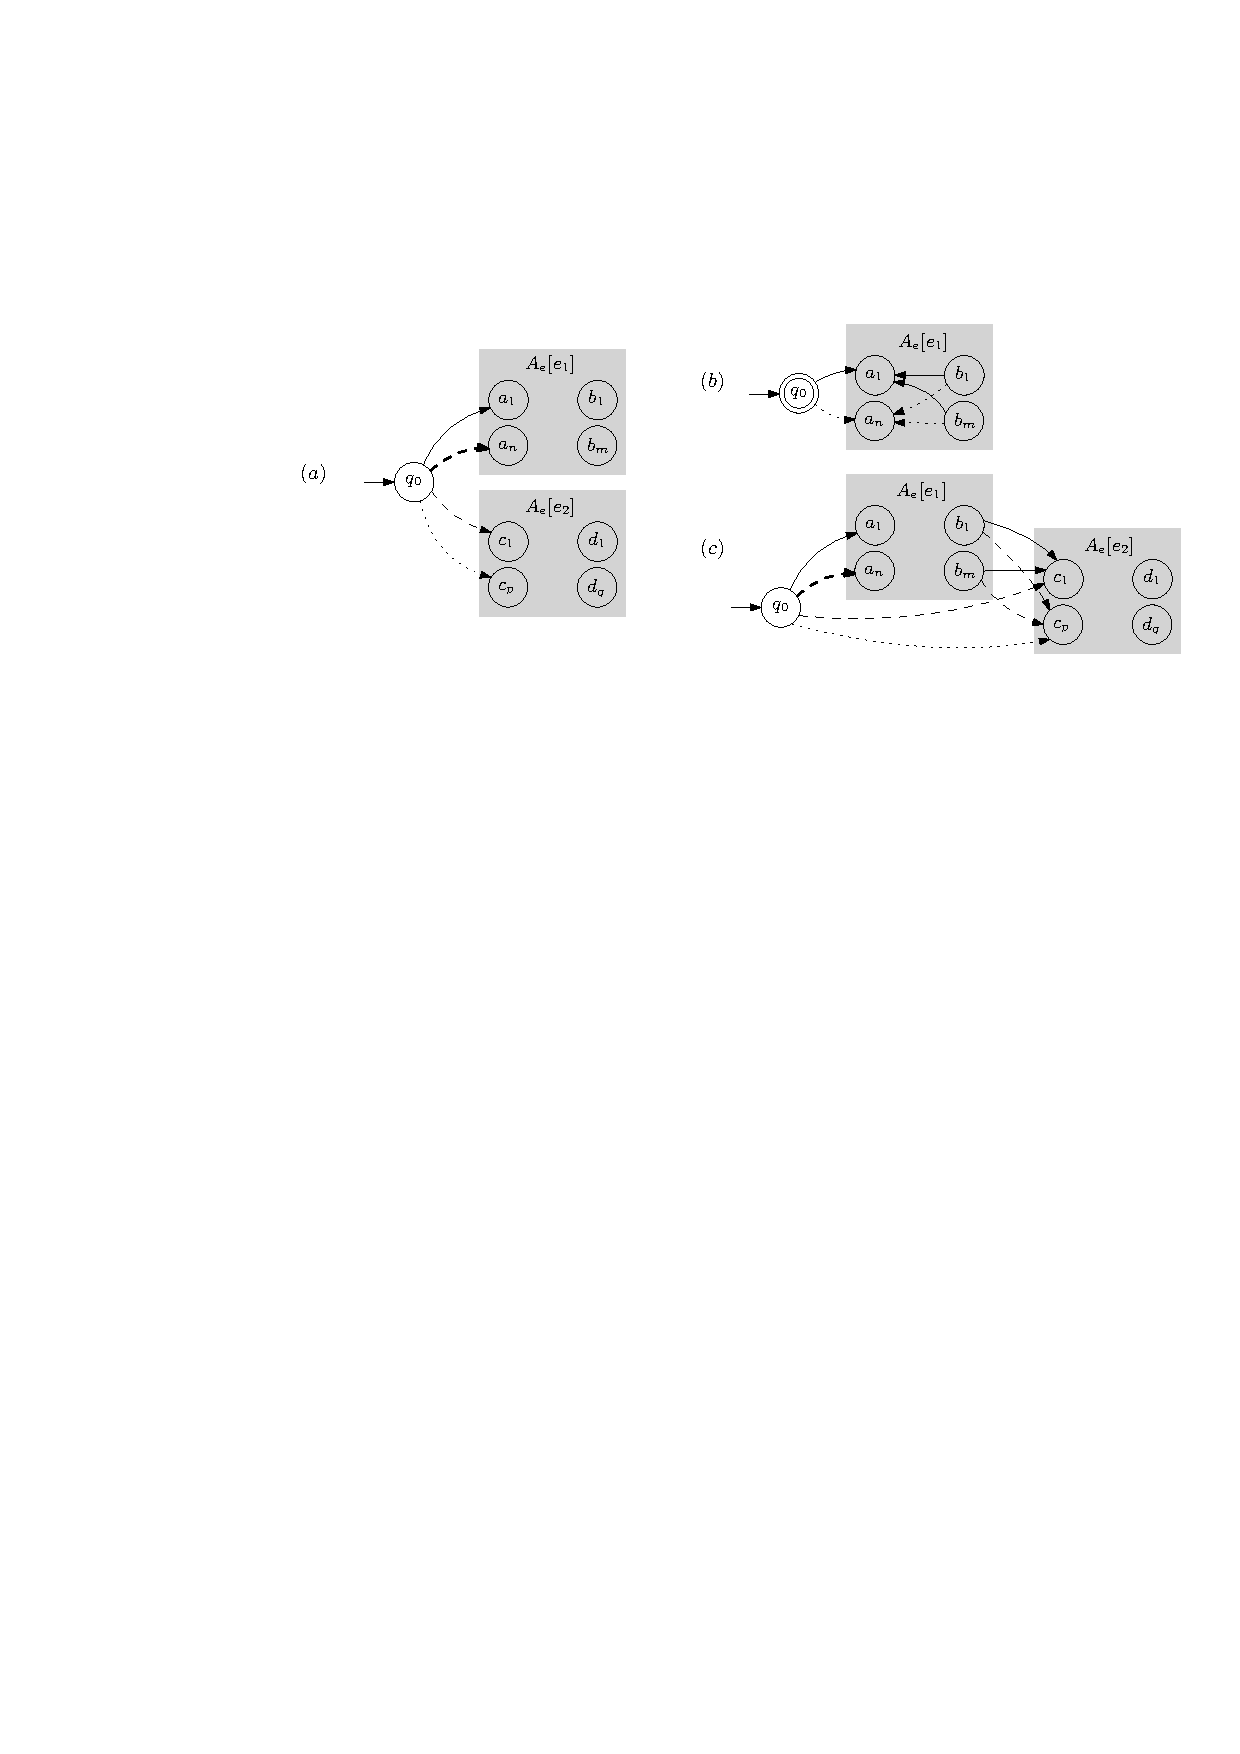
\includegraphics{pglushkov_01}
%	\caption{pNFA $A_e$ for (a) $e=e_1+e_2$ (b) $e=e_1^{\ast}$ and (c) $e=e_1 \concat e_2$ where $\varepsilon \in \Lang(e_1)$ and $\varepsilon \notin \Lang(e_2)$. A transition of lower priority is depicted thiner and more densely dotted. }
%	\label{fig:pglushkov}
%\end{figure*}

For any $e \in \regexp[\sf CG]$, a PFA $\cA_e$ can be constructed recursively by adapting the standard
Thompson construction (cf. Section 4.1 in \cite{Thompson68}). The constructed PFA $\cA_e$ satisfies that it has a unique initial state without incoming transitions and a unique final state  without outgoing transitions.
%The original construction on regular expressions
%produces an FA without $\varepsilon$-transitions, which we denote by $G_e$.
%We refer the reader to \cite{Gluskov61} for 
%details of how to construct $G_e$. %\tl{is this just the textbook construction?}
%
%The pNFA $A_e$ is obtained by recursively adding priority to $G_e$ as follows:
\begin{itemize}
\item If $e =\emptyset$, then $\cA_e = (\{q_0,f_0\}, \Sigma, \delta, \tau, q_0, f_0)$, where $\delta(q_0, \sigma) = \delta(f_0, \sigma) = ()$ for every $\sigma \in \Sigma$, $\tau(q_0) = \tau(f_0)= ((); ())$.

  \item If $e = \varepsilon$, then  $\cA_e = (\{q_0, f_0\}, \Sigma, \delta, \tau, q_0, f_0)$, where  $\delta(q_0, \sigma) = \delta(f_0, \sigma) = ()$ for every $\sigma \in \Sigma$, $\tau(q_0) = ((f_0); ())$, and $\tau(f_0) = ((); ())$. 

  \item If $e = a$, then $\cA_e = (\{q_0, f_0\}, \Sigma, \delta, \tau, q_0, f_0)$, where  $\delta(q_0, a) = (f_0)$, $\delta(q_0, \sigma) = ()$ for every $\sigma \in \Sigma \setminus \{a\}$, $\tau(q_0) = ((); ())$, and $\tau(f_0) = ((); ())$.
    
  \item If $e = (e_1)$, then $\cA_e = \cA_{e_1}$.
  
  \item If $e = e_1 + e_2$, and suppose $\cA_{e_1} = (Q_1,
  \Sigma, \delta_1, \tau_1, q_1, f_1)$ and $\cA_{e_2} = (Q_2, \Sigma,
  \delta_2, \tau_2, q_2, f_2)$, then $\cA_e = (Q_1 \cup Q_2 \cup \{q_0, f_0\}, \Sigma,
  \delta, \tau, q_0, f_0)$, where  
  \begin{itemize}
 \item $q_0, f_0 \not \in Q_1 \cup Q_2$, 
 \item $\delta(q) = \delta_i(q)$ for every $q \in Q_i$ ($i=1,2$), 
$\delta(q_0, \sigma) = \delta(f_0, \sigma) = ()$ for every $\sigma \in \Sigma$, 
%
 \item $\tau(q) = \tau_i(q)$ for every $q \in Q_i$ ($i =1,2$), $\tau(q_0) = ((q_1,q_2); ())$,  $\tau(f_1) = \tau(f_2) = ((f_0); ())$, and $\tau(f_0) = ((); ())$.
 \end{itemize}
%
  \item If $e = e_1 \concat e_2$, and suppose $\cA_{e_1} = (Q_1,
  \Sigma, \delta_1, \tau_1, q_1, f_1)$ and $\cA_{e_2} = (Q_2, \Sigma,
  \delta_2, \tau_2, q_2, f_2)$, then $\cA_e = ( Q_1 \cup Q_2, \Sigma, \delta, \tau, q_1,
  f_2)$, where 
  \begin{itemize}
    \item for every $q \in Q_i$, $\delta(q) = \delta_i(q)$ ($i = 1,2$),
    
    \item for every $q \in Q_2$, $\tau(q) = \tau_2(q)$, 
%
    \item for every $q \in Q_1 \setminus \{f_1\}$, $\tau(q) = \tau_1(q)$, and $\tau(f_1) = ((q_2); ())$.
  \end{itemize}
%  
  \item If $e = e_1^{\ast}$, and suppose  $\cA_{e_1} = (Q_1,
  \Sigma, \delta_1, \tau_1, q_1, f_1)$, then $\cA_e = (Q_1 \cup \{q_0, f_0\}, \Sigma,
  \delta, \tau, q_0, f_0)$, where 
  \begin{itemize}
  \item $q_0, f_0 \not \in Q_1$,
  
    \item for every $q \in Q_1$ and $\sigma \in \Sigma$, $\delta(q, \sigma) = \delta_1(q, \sigma)$, moreover, $\delta(q_0, \sigma) = \delta(f_0, \sigma)  = ()$,
    
    \item for every $q \in Q_1 \setminus \{f_1\}$,  $\tau(q) = \tau_1(q)$, moreover, $\tau(q_0) = ((q_1, f_0); ())$, $\tau(f_1) = ((q_1, f_0); ())$, and $\tau(f_0) = ((); ())$.
  \end{itemize}
 %
  \item If $e = e_1^{\ast?}$, and suppose $\cA_{e_1} = (Q_1,
  \Sigma, \delta_1, \tau_1, q_1, f_1)$, then $\cA_e = (Q_1 \cup \{q_0, f_0\}, \Sigma,
  \delta, \tau, q_0, f_0)$, where 
  \begin{itemize}
  \item $q_0, f_0 \not \in Q_1$,
  
    \item for every $q \in Q_1$ and $\sigma \in \Sigma$, $\delta(q, \sigma) = \delta_1(q, \sigma)$, moreover, $\delta(q_0, \sigma) = \delta(f_0, \sigma)  = ()$,
    
    \item for every $q \in Q_1 \setminus \{f_1\}$,  $\tau(q) = \tau_1(q)$, moreover, $\tau(q_0) = ((f_0, q_1); ())$, $\tau(f_1) = ((f_0, q_1); ())$, and $\tau(f_0) = ((); ())$.
  \end{itemize}  
\end{itemize}

%The key transitions of some non-trivial cases of the construction are illustrated in Figure.\ref{fig:pglushkov}.

% An important property of the automaton $G_e$ and thus $A_e$ is that, for any subexpression $e'$ of $e$, there must be a subgraph of $A_{e}$ corresponding to $e'$. We denote this subgraph by $A_{e}[e']$. This subgraph can be seen as the automaton obtained by removing from $A_{e'}$ the state $q_0$ and all transitions from it.

\begin{example}
Let $e_1 = a^\ast$ and $e_2 = a^{\ast ?}$. Then the PFAs $\cA_{e_1} = (Q_1, \Sigma, \delta_1, \tau_1, q_0, q_3)$ and $\cA_{e_2} =  (Q_2, \Sigma, \delta_2, \tau_2, q_0, q_3)$ are illustrated in Figure~\ref{fig-retopfa}: (i), (ii), where thicker solid lines denote the $\varepsilon$-transitions of greater priorities. For instance, in $\cA_{e_1}$, $\tau_1(q_0) = ((q_1, q_3); ())$ and $\tau_1(q_2) = ((q_1, q_3); ())$, while in $\cA_{e_2}$, $\tau_2(q_0) = ((q_3, q_1); ())$ and $\tau_2(q_2) = ((q_3, q_1); ())$. Note that $\cA_{e_1}$ and $\cA_{e_2}$ are different from those in Example~\ref{exmp-pfa}.
\begin{figure}[ht]
\centering
%\rule{\linewidth}{0cm}
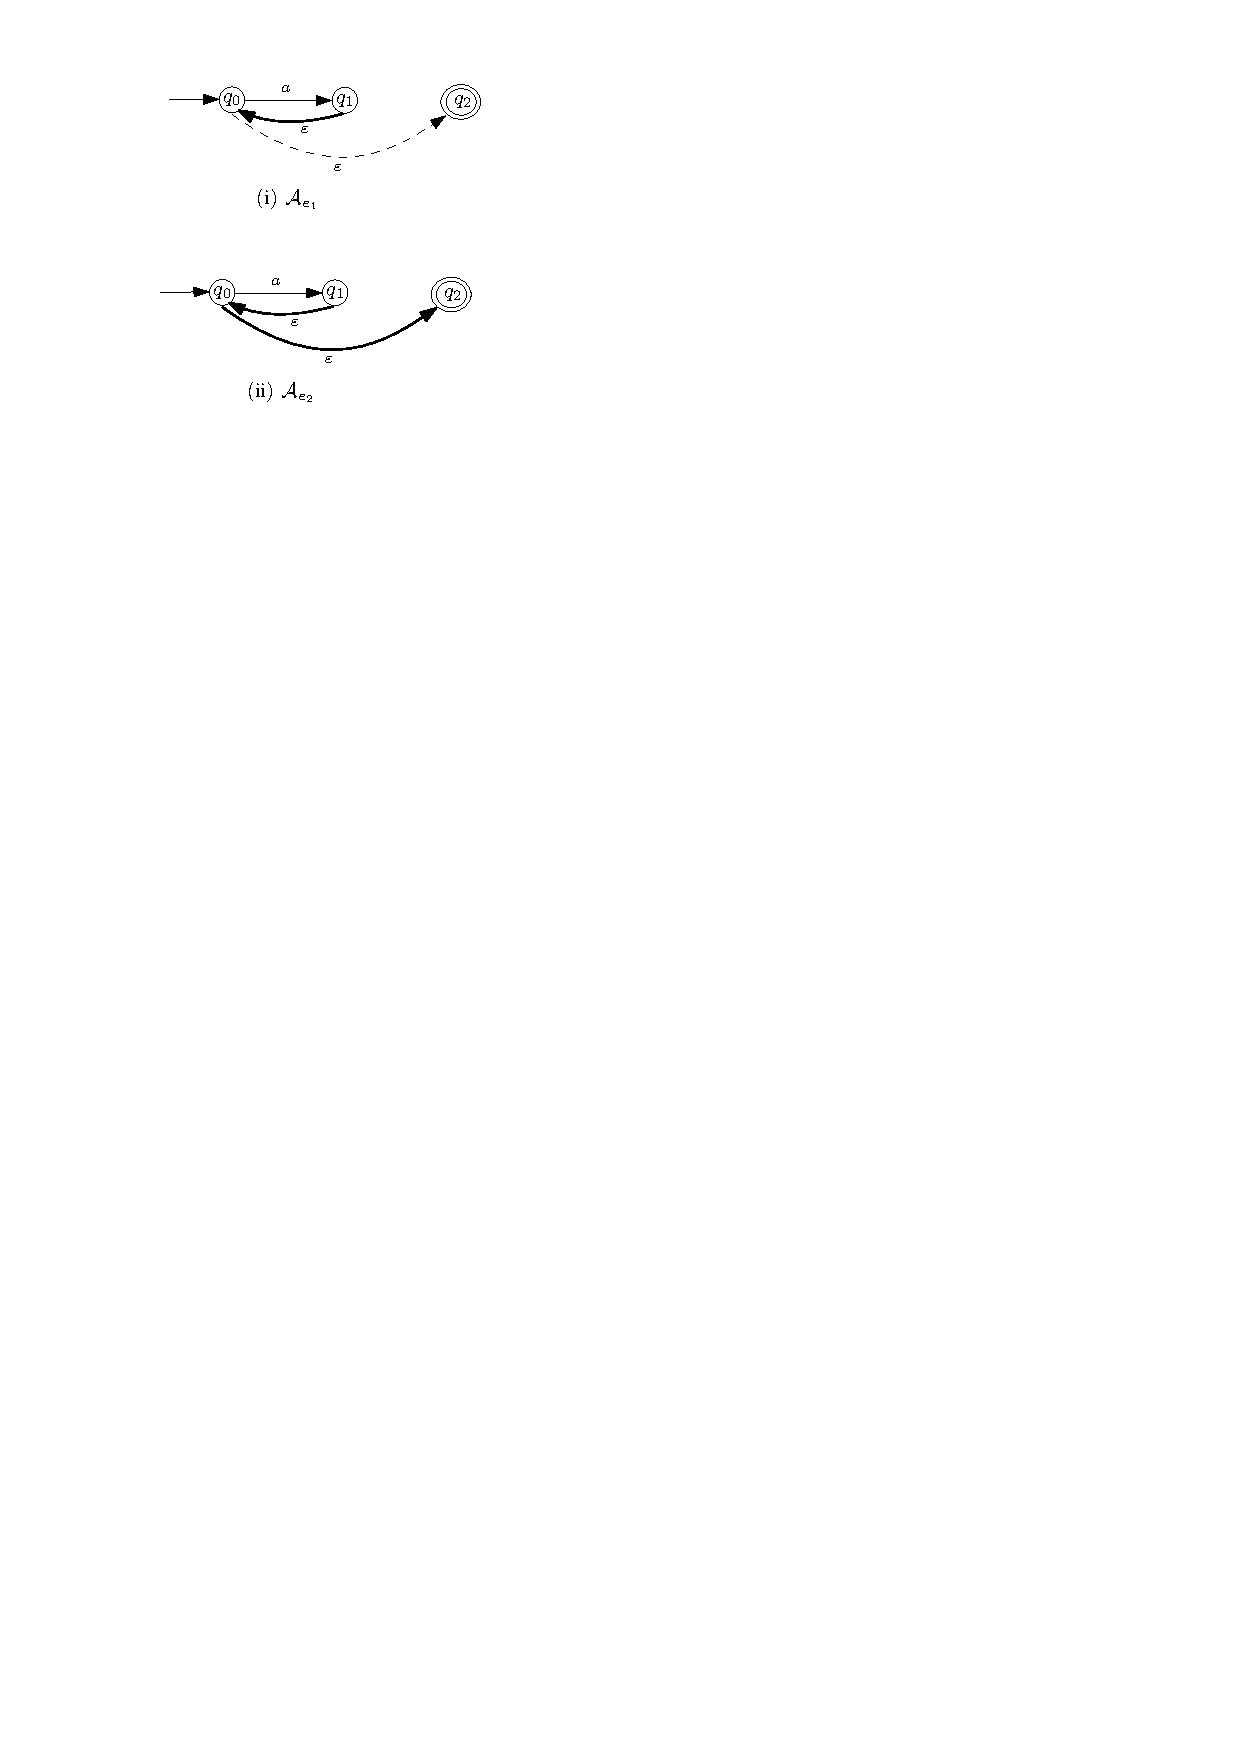
\includegraphics[scale=0.8]{retopfa.pdf}
\caption{$\cA_{e_1}$ and $\cA_{e_2}$ for $e_1= a^\ast$ and $e_2 = a^{\ast?}$}
\label{fig-retopfa}
\end{figure}
\end{example}
 
%For instance, if $e = (a (ab)^*)^*$ and $e' = a(ab)^*$, then $A_{e}[e']$ is the subgraph of $A_{e}$ comprising the states $\{a_1, a_2, b_3\}$ and the transitions $\{(a_1, a, a_2), (a_2, b, b_3), (b_3, a, a_2)\}$.
 
%Figure.\ref{fig:pglushkov} also illustrates the subgraphs corresponding to direct subexpressions of $e$.


%\begin{definition}
%Let $e \in \regexp[\sf CG]$ and $e'$ be a subexpression of $e$. Then a copy of $\cA_{e'}$ in $\cA_e = (Q, \Sigma, \delta, \tau, q_0, f_0)$ is a PFA $(Q', \Sigma, \delta', \tau', q'_0, f'_0)$ such that  
%\begin{itemize}
%\item $Q' \subseteq Q$, $q'_0, f'_0 \in Q'$, 
%\item $\delta'$ is the restriction of $\delta$ to $Q'$, with the outgoing transitions of $f'_0$ removed, specifically, for every $\sigma \in \Sigma$ and $q \in Q' \setminus \{f'_0\}$, $\delta'(q, \sigma) = \delta(q, \sigma)$, $\tau'(q) = \tau(q)$, $\delta'(f'_0, \sigma) = ()$, and $\tau'(f'_0) = ((); ())$,
%\item $(Q', \Sigma, \delta', \tau', q'_0, f'_0)$ is isomorphic to $\cA_{e'}$.
%\end{itemize}
%\end{definition}

From the aforementioned recursive construction of $\cA_e$, we know that for each subexpression $e'$ of $e$, a PFA for $e'$, which is isomorphic to $\cA_{e'}$, is also constructed. Let us use ${\sf Sub}_{e'}[\cA_e]$ to denote this PFA for $e'$, which, roughly speaking, is a subgraph of $\cA_e$.
%\begin{proposition}\label{prop-subexp}
%Let $e \in \regexp[\sf CG]$. Then for every subexpression $e'$ of $e$, there is a unique copy of $\cA_{e'}$ in $\cA_e$, denoted by ${\sf Sub}_{e'}[\cA_e]$.
%\end{proposition}

%\begin{definition}
%  Let $A_e$ be the pNFA constructed for $e$, and $p = q_0 \sigma_1 q_1 \ldots
%  \sigma_m q_m$ is the accepting run of $A_e$ on string w. For any subexpression $e'$ of $e$, we say a
%  consecutive sequence of states $q_i q_{i + 1} \ldots q_{j - 1} q_j$ in p is
%  a maximal $e'$-match, if $q_i \in \tmop{Start} (e')$, $q_j \in \tmop{End}
%  (e')$, $(q_{i - 1}, \sigma_i, q_i)$ is not a transition in $A_e [e']$, and
%  for any $k \in [i, j]$, $q_k$ is a vertex in $A_e [e']$. Moreover, if $j
%  \neq m$, then $(q_j, \sigma_{j + 1}, q_{j + 1})$ is not a transition in $A_e
%  [e']$.
  
%  We use $p_{e', e} (w)$ to denote the sequence of disjoint maximal $e'$-match
%  $w_1 \ldots w_n$, in the order they occur in p. Note that in $A_e$, all
%  states except $q_0$ are labeled by a letter, thus a maximal $e'$-match can
%  be seen as a string.
%\end{definition}

%The following  theorem states the equivalence of the accepting match of a \regexp[\sf CG] $e$ and the accepting run of $A_e$ on the same input string, thus the construction precisely captures the semantics. % in \ref{semantics:regex}.
%\begin{theorem}
% \label{theorem:regex_pnfa_equiv}
%  For any regular expression e, subexpression $e'$ of e, and $w \in L (e)$,
%  $m_{e', e} (w) = p_{e', e} (w)$
%\end{theorem}
%
%For simplicity, we refer the reader to the appendix for proof.


 
\subsection{Proof of Lemma~\ref{lem-extract}-\ref{lem-replace}}

We first prove Lemma~\ref{lem-extract}, namely, show how to construct a PPST $\cT_{\extract_{i,e}}$ for $\extract_{i,e}$.

\paragraph*{Construction of $\cT_{\extract_{i,e}}$.} 
Let $e'$ be the subexpression corresponding to the $i$-th capturing group of $e$. In particular, if $i=0$, then $e' = e$. 

Suppose $\cA_e = (Q, \Sigma, \delta, \tau, q_0, f_0)$. Then $\cT_{\extract_{i,e}} = (Q \cup \{q'_0, f'_0\}, \Sigma, X, \delta', \tau', E, q'_0, F)$ where
\begin{itemize}
\item $q'_0, f'_0 \not \in Q$,

\item  $X = \{x\}$,
%
\item $F(f'_0) = x$, and $F(q')$ is undefined for every $q' \in Q \cup \{q'_0\}$,

\item $\delta'$ and $\tau'$ are obtained from $\delta$ and $\tau$ as follows,
\begin{itemize}
\item $\delta'(q'_0, \sigma) = (q'_0)$ for every $\sigma \in \Sigma$, and $\tau'(q'_0) = ((q_0); ())$,
%
\item  for every $q \in Q \setminus \{f_0\}$ and $\sigma \in \Sigma$, $\delta'(q, \sigma) = \delta(q, \sigma)$ and $\tau'(q) = \tau(q)$, 
%
\item $\delta'(f_0, \sigma) = ()$ for every $\sigma \in \Sigma$ and $\tau'(f_0) = ((f'_0); ())$,
%
\item $\delta'(f'_0, \sigma) = (f'_0)$ for every $\sigma \in \Sigma$ and $\tau'(f'_0) = ((); ())$,
\end{itemize}
%
\item $E$ is defined as follows, 
\begin{itemize}
\item for every transition $(q, \sigma, q')$ with  $\sigma \in \Sigma^\varepsilon$ in ${\sf Sub}_{e'}[\cA_e]$, we have $E(q, \sigma, q')(x) = x\sigma$, 
\item for all the other transitions $(q, \sigma, q')$ with $\sigma \in \Sigma^\varepsilon$ in $\cA_e$, we have $E(q, \sigma, q')(x) = x$, 
\item $E(q'_0, \sigma, q'_0)(x) = x$ for every $\sigma \in \Sigma$, $E(q'_0, \varepsilon, q_0)(x) = x$, 
\item $E(f_0, \varepsilon, f'_0)(x) = x$, and $E(f'_0, \sigma, f'_0)(x) = x$ for every $\sigma \in \Sigma$.
\end{itemize}
%
\end{itemize}



\paragraph*{Construction of $\cT_{\replaceall_{\pat, \rep}}$.} 
Let $\$i_1, \cdots, \$i_k$ with $i_1 < \cdots < i_k$ be an enumeration of all the references in $\rep$. 
Moreover, for every $j \in [k]$, let $e'_{i_j}$ be the subexpression of $\pat$ corresponding to the $i_j$-th capturing group.
Suppose $\cA_\pat = (Q, \Sigma, \delta, \tau, q_0, f_0)$. Then $\cT_{\replaceall_{\pat, \rep}} =$ $(Q \cup \{q'_0, f'_0\}$, $\Sigma$, $X$, $\delta'$, $\tau', E, q'_0, F)$ where
\begin{itemize}
\item $q'_0, f'_0 \not \in Q$,

\item  $X = \{x_0, x_1, \cdots, x_k\}$,
%
\item $F(f'_0) = x_0$, and $F(q')$ is undefined for every $q' \in Q \cup \{q'_0\}$,
%
\item $\delta'$ and $\tau'$ are obtained from $\delta$ and $\tau$ as follows,
\begin{itemize}
\item $\delta'(q'_0, \sigma) = (q'_0)$ for every $\sigma \in \Sigma$, and $\tau'(q'_0) = ((q_0); ())$,
%
\item  for every $q \in Q \setminus \{f_0\}$ and $\sigma \in \Sigma$, $\delta'(q, \sigma) = \delta(q, \sigma)$ and $\tau'(q) = \tau(q)$, 
%
\item $\delta'(f_0, \sigma) = ()$ for every $\sigma \in \Sigma$ and $\tau'(f_0) = ((q'_0,f'_0); ())$,
%
\item $\delta'(f'_0, \sigma) = (f'_0)$ for every $\sigma \in \Sigma$ and $\tau'(f'_0) = ((); ())$.
\end{itemize}
%
\item $E$ is defined as follows, 
\begin{itemize}
\item for every transition $(q, \sigma, q')$ with $\sigma \in \Sigma^\varepsilon$ in $\cA_\pat$, $E(q, \sigma, q')(x_0) = x_0$,
%
\item for every transition $(q, \sigma, q')$ with $\sigma \in \Sigma^\varepsilon$ and every $j \in [k]$,  if $(q, \sigma, q')$ occurs in ${\sf Sub}_{e'_{i_j}}[\cA_\pat]$, then $E(q, \sigma, q')(x_j) = x_j\sigma$, otherwise, $E(q, \sigma, q')(x_j) = x_j$,
%
%\item for all the other transitions $(q, \sigma, q')$ with $\sigma \in \Sigma^\varepsilon$ in $\cA_e$, we have $E(q, \sigma, q')(x) = x$, 
%
\item  for every $\sigma \in \Sigma$, $E(q'_0, \sigma, q'_0)(x_0) = x_0\sigma$, and for every $j \in [k]$, $E(q'_0, \sigma, q'_0)(x_j) = x_j$, 

\item $E(q'_0, \varepsilon, q_0)(x_j) = x_j$ for every $j \in [k] \cup \{0\}$, 
%
\item $E(f_0, \varepsilon, q'_0)(x_0) = x_0 \rep[x_1/\$i_1,\ldots, x_k/\$i_k]$, and for every $j \in [k]$, $E(f_0, \varepsilon, q'_0)(x_j) = \varepsilon$, 
%
\item $E(f_0, \varepsilon, f'_0)(x_0) = x_0  \rep[x_1/\$i_1,\ldots, x_k/\$i_k]$, and for every $j \in [k]$, $E(f_0, \varepsilon, f'_0)(x_j) = \varepsilon$,
%
\item for every $\sigma \in \Sigma$, $E(f'_0, \sigma, f'_0)(x_0) = x_0$, and  for every $j \in [k]$, $E(f'_0, \sigma, f'_0)(x_j) = x_j$.
\end{itemize}
%
\end{itemize}

\zhilin{stopped here}

\subsection{Complexity}

\begin{proposition}[POPL'19]
	The path feasibility problem of the following two fragments is non-elementary: SL with 2FTs, and SL with FTs+replaceAll.
	
	SL[conc, replaceAll, reverse, FFT] is expspace-complete (note that 2FTs in SL are restricted to be one-way and functional)
\end{proposition}

%The same proof strategy can be used for FTs+replaceAll. The 2FTs used in the proof above
%proceed by running completely over the word and producing some output, then silently moving
%back to the beginning of the word. An arbitrary number of passes are made in this way. We
%can simulate this behaviour using FTs and replaceAll.


The main open question is the complexity of the SL fragment with replaceall function and prioritized streaming transducers. Note that PSST can simulate 2FT (adapting Matt's proof?), so we could obtain nonelementary lower bound for SL with PSST.

However, this variant of replaceall is quite different from the replaceall we had before ...

\begin{enumerate}
\item  does  copyless help?
\item how about SL with only this version of replaceall?
\end{enumerate}
